% !TeX program = xelatex
\documentclass[a4paper,10pt]{article}

% ============================================================================
% កញ្ចប់បណ្ណាល័យ (Packages) – តាមលំនាំ ករណី ម.ជ.ម (ls_plan.tex)
% ============================================================================
\usepackage[a4paper, left=0.95cm, right=0.95cm, top=0.85cm, bottom=0.92cm, footskip=0.52cm]{geometry}
\usepackage{amsmath}
\usepackage{unicode-math}
\usepackage{fontspec}
\usepackage{array, longtable, multirow, colortbl}
\usepackage[table]{xcolor}
\usepackage{enumitem}
\usepackage{pifont}
\usepackage{fancyhdr}
\usepackage{tikz}
\usetikzlibrary{calc, arrows.meta, angles, quotes, decorations.markings, babel}

% LaTeX 2025 + longtable v4.24 compatibility guard
\makeatletter
\let\@expl@@@mark@update@singlecol@structures@@\relax
\makeatother

% ============================================================================
% ការកំណត់ពុម្ពអក្សរ (Fonts Configuration) – តាមលំនាំ ម.ជ.ម ១០០%
% ============================================================================
% Cross-platform font path resolver (Windows local + Linux/Cloud repo fonts/)
\providecommand{\NGSFindFonts}{%
  \IfFileExists{C:/Windows/Fonts/cambria.ttc}{%
    \def\NGSSysPath{C:/Windows/Fonts/}%
    \def\NGSUserPath{C:/Users/KIT/AppData/Local/Microsoft/Windows/Fonts/}%
  }{%
    \IfFileExists{./fonts/KhmerOSsiemreap.ttf}{\def\NGSSysPath{./fonts/}\def\NGSUserPath{./fonts/}}{%
    \IfFileExists{../fonts/KhmerOSsiemreap.ttf}{\def\NGSSysPath{../fonts/}\def\NGSUserPath{../fonts/}}{%
    \IfFileExists{../../fonts/KhmerOSsiemreap.ttf}{\def\NGSSysPath{../../fonts/}\def\NGSUserPath{../../fonts/}}{%
    \IfFileExists{../../../fonts/KhmerOSsiemreap.ttf}{\def\NGSSysPath{../../../fonts/}\def\NGSUserPath{../../../fonts/}}{%
    \IfFileExists{../../../../fonts/KhmerOSsiemreap.ttf}{\def\NGSSysPath{../../../../fonts/}\def\NGSUserPath{../../../../fonts/}}{%
    \IfFileExists{../../../../../fonts/KhmerOSsiemreap.ttf}{\def\NGSSysPath{../../../../../fonts/}\def\NGSUserPath{../../../../../fonts/}}{%
    \IfFileExists{../../../../../../fonts/KhmerOSsiemreap.ttf}{\def\NGSSysPath{../../../../../../fonts/}\def\NGSUserPath{../../../../../../fonts/}}{%
      \def\NGSSysPath{../../../../../../../fonts/}\def\NGSUserPath{../../../../../../../fonts/}%
    }}}}}}}%
  }%
}
\NGSFindFonts

\setmathfont[
  Path={\NGSSysPath},
  FontIndex=1,
  Scale=1.02
]{cambria.ttc}

\defaultfontfeatures{Ligatures=TeX}

\setmainfont[
  Path={\NGSUserPath},
  Extension=.ttf,
  Script=Khmer,
  BoldFont={KhmerOSsiemreap},
  BoldFeatures={FakeBold=1.8},
  ItalicFont={KhmerOSsiemreap},
  ItalicFeatures={FakeSlant=0.25},
  BoldItalicFont={KhmerOSsiemreap},
  BoldItalicFeatures={FakeBold=1.8, FakeSlant=0.25}
]{KhmerOSsiemreap}

\newfontfamily\muol[
  Path={\NGSUserPath},
  Extension=.ttf,
  Script=Khmer
]{KhmerOSmuollight}

\newfontfamily\NagaBold[
  Path={\NGSUserPath},
  Extension=.ttf
]{AKbalthom Naga Bold}

\newfontfamily\CalibriFont[
  Path={\NGSSysPath},
  Extension=.ttf
]{calibri}

\newfontfamily\Tacteing[
  Path={\NGSUserPath}
]{TACTENG.TTF}

\newfontfamily\CourierBullet[
  Path={\NGSSysPath},
  Extension=.ttf
]{cour}
\newcommand{\wcirc}{{\CourierBullet\fontsize{9.5pt}{11pt}\selectfont o}}

% ក្បួនកាត់ពាក្យខ្មែរ (Khmer word wrapping)
\XeTeXlinebreaklocale "km"
\XeTeXlinebreakskip = 0pt plus 1pt minus 0.1pt

% ============================================================================
% ការកំណត់ពណ៌ និងទម្រង់ទំព័រ (Colors & Page Style)
% ============================================================================
\definecolor{stepgray}{HTML}{D9D9D9}
\definecolor{headgray}{HTML}{F2F2F2}
\definecolor{boxgray}{HTML}{D9D9D9}
\definecolor{darkred}{HTML}{C00000}
\definecolor{red5e}{HTML}{FF0000}
\definecolor{triblue}{HTML}{DAE8FC}
\definecolor{triborders}{HTML}{6C8EBF}
\definecolor{arrowblue}{HTML}{4472C4}
\definecolor{figblue}{HTML}{1F4E9E}
\definecolor{tealink}{HTML}{0F766E}
\definecolor{amberwarm}{HTML}{D97706}
\definecolor{pondcyan}{HTML}{DDF3FA}
\definecolor{pondstroke}{HTML}{0E7490}

\pagestyle{fancy}
\fancyhf{}
\renewcommand{\headrulewidth}{0pt}
\fancyfoot[R]{\CalibriFont\fontsize{11pt}{13pt}\selectfont\thepage}

\setlength{\parindent}{0pt}
\setlength{\parskip}{0pt}
\setlength{\tabcolsep}{3.8pt}

\newcolumntype{L}[1]{>{\raggedright\arraybackslash}p{#1}}

% ============================================================================
% ម៉ាក្រូជំនួយ (Helper Macros) – តាមលំនាំ ម.ជ.ម
% ============================================================================
\newcommand{\fiveE}[1]{{\NagaBold\fontsize{10pt}{14pt}\selectfont\textcolor{red5e}{#1}}}
\newcommand{\timenote}[1]{\textcolor{darkred}{\textit{#1}}}
\newcommand{\redsub}[1]{\textcolor{darkred}{#1}}
\newcommand{\graybox}[1]{\colorbox{boxgray}{\strut\hspace{2pt}#1\hspace{2pt}}}
\newcommand{\ditem}{\tikz[baseline=-0.5ex]\fill (0,0.42ex) -- (0.42ex,0) -- (0,-0.42ex) -- (-0.42ex,0) -- cycle;\hspace{0.3em}}
\newcommand{\cnum}[1]{{\fontsize{10.5pt}{12pt}\selectfont\ding{\numexpr181+#1\relax}}\hspace{0.2em}}
\newcommand{\cfig}[1]{\par\vspace{4pt}{\centering #1\par}\vspace{4pt}}
\newcommand{\stepheader}[1]{\multicolumn{3}{|c|}{\cellcolor{stepgray}\muol #1} \\* \noalign{\hrule height 0.4pt}}
\newcommand{\tri}[1]{\ensuremath{\triangle #1}}
\newcommand{\ang}[1]{\ensuremath{\angle #1}}
\newcommand{\cg}{\ensuremath{\cong}}

% រចនាប័ទ្មគូសសម្គាល់ជ្រុងស្មើគ្នា (Tick mark styles - bold B&W print safe)
\tikzset{
  tk1/.style={postaction={decorate},decoration={markings,mark=at position 0.50 with {\draw[black, line width=0.85pt](0,-0.095)--(0,0.095);}}},
  tk2/.style={postaction={decorate},decoration={markings,
    mark=at position 0.45 with {\draw[black, line width=0.85pt](0,-0.095)--(0,0.095);},
    mark=at position 0.55 with {\draw[black, line width=0.85pt](0,-0.095)--(0,0.095);}}}
}

% ក្បាច់ក្រោមបាវចនា (Tacteing Font - Keyboard '3')
\newcommand{\khmflourish}{{\Tacteing\fontsize{36pt}{14pt}\selectfont\raisebox{-5pt}{3}}}

% ============================================================================
% ម៉ាក្រូគូសរូបធរណីមាត្រ (Reusable TikZ Geometric Macros)
% ============================================================================

% ១. កំណែកិច្ចការផ្ទះមេរៀនមុន (ម.ជ.ម) – ស-ខ្មៅ បន្ទាត់ច្បាស់
\newcommand{\figHWold}{%
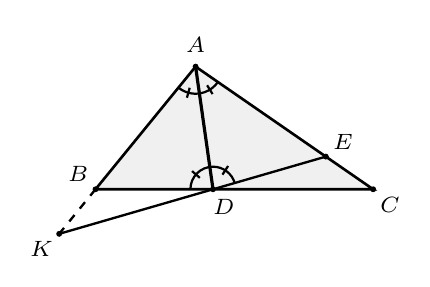
\begin{tikzpicture}[scale=0.82, every node/.style={font=\footnotesize, text=black}]
  \coordinate (A) at (0, 1.90);
  \coordinate (B) at (-1.55, 0);
  \coordinate (C) at (2.75, 0);
  \coordinate (D) at (0.2696, 0);
  \coordinate (E) at (2.0174, 0.5062);
  \coordinate (K) at (-2.1129,-0.6900);
  \fill[gray!12] (A) -- (B) -- (C) -- cycle;
  \draw[black, line width=0.95pt] (A) -- (B) -- (C) -- cycle;
  \draw[black, line width=0.85pt, dashed] (B) -- (K);
  \draw[black, line width=1.15pt] (A) -- (D);
  \draw[black, line width=0.85pt] (E) -- (K);
  \draw[black, line width=0.8pt] ($(A)+(-129.21:0.42)$) arc (-129.21:-34.64:0.42);
  \draw[black, line width=0.8pt] ($(A)+(-105.57:0.34)$) -- ($(A)+(-105.57:0.50)$);
  \draw[black, line width=0.8pt] ($(A)+(-58.28:0.34)$) -- ($(A)+(-58.28:0.50)$);
  \draw[black, line width=0.8pt] ($(D)+(180:0.35)$) arc (180:16.15:0.35);
  \draw[black, line width=0.8pt] ($(D)+(139.04:0.27)$) -- ($(D)+(139.04:0.43)$);
  \draw[black, line width=0.8pt] ($(D)+(57.11:0.27)$) -- ($(D)+(57.11:0.43)$);
  \fill[black] (A) circle (1.3pt) node[above=1.5pt] {$A$};
  \fill[black] (B) circle (1.3pt) node[above left=1.5pt, inner sep=1pt] {$B$};
  \fill[black] (C) circle (1.3pt) node[below right=1.5pt, inner sep=1pt] {$C$};
  \fill[black] (D) circle (1.3pt) node[below=2.5pt, xshift=4pt, inner sep=1pt] {$D$};
  \fill[black] (E) circle (1.3pt) node[above right=1.5pt, inner sep=1pt] {$E$};
  \fill[black] (K) circle (1.3pt) node[below left=1.5pt, inner sep=1pt] {$K$};
\end{tikzpicture}}

% ២. រំលឹកមុំទល់កំពូល & កន្លះបន្ទាត់ពុះមុំ – ស-ខ្មៅ បន្ទាត់ច្បាស់
\newcommand{\figVert}{%
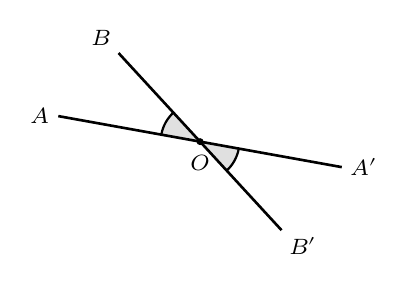
\begin{tikzpicture}[scale=0.90, every node/.style={font=\footnotesize, text=black}]
  \coordinate (O) at (0,0);
  \coordinate (A) at (-2.00, 0.36);
  \coordinate (Ap) at (2.00, -0.36);
  \coordinate (B) at (-1.15, 1.25);
  \coordinate (Bp) at (1.15, -1.25);
  \pic[draw=black, line width=0.8pt, fill=gray!24, angle radius=5.0mm]{angle=B--O--A};
  \pic[draw=black, line width=0.8pt, fill=gray!24, angle radius=5.0mm]{angle=Bp--O--Ap};
  \draw[black, line width=0.95pt] (A) -- (Ap);
  \draw[black, line width=0.95pt] (Bp) -- (B);
  \fill[black] (O) circle (1.4pt);
  \node[left=2pt, inner sep=1pt] at (A) {$A$};
  \node[right=2pt, inner sep=1pt] at (Ap) {$A'$};
  \node[above left=1.5pt, inner sep=1pt] at (B) {$B$};
  \node[below right=1.5pt, inner sep=1pt] at (Bp) {$B'$};
  \node[below=3.5pt, inner sep=1pt] at (O) {$O$};
\end{tikzpicture}}

\newcommand{\figBisect}{%
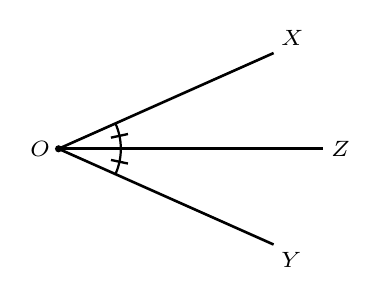
\begin{tikzpicture}[scale=0.92, every node/.style={font=\footnotesize, text=black}]
  \coordinate (O) at (0,0);
  \coordinate (X) at (24:3.25);
  \coordinate (Y) at (-24:3.25);
  \coordinate (Z) at (3.65,0);
  \draw[black, line width=0.95pt] (O) -- (X) (O) -- (Y);
  \draw[black, line width=1.15pt] (O) -- (Z);
  \draw[black, line width=0.8pt] (24:0.86) arc (24:-24:0.86);
  \draw[black, line width=0.85pt] (12:0.74) -- (12:0.98);
  \draw[black, line width=0.85pt] (-12:0.74) -- (-12:0.98);
  \fill[black] (O) circle (1.4pt) node[left=2pt, inner sep=1pt] {$O$};
  \node[above right=1.5pt, inner sep=1pt] at (X) {$X$};
  \node[below right=1.5pt, inner sep=1pt] at (Y) {$Y$};
  \node[right=2pt, inner sep=1pt] at (Z) {$Z$};
\end{tikzpicture}}

% ៣. E1 Engage: បេសកកម្មវាស់ទទឹងស្រះទឹក – ស-ខ្មៅ បន្ទាត់ច្បាស់
\newcommand{\figPondHook}{%
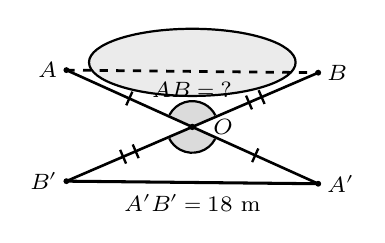
\begin{tikzpicture}[scale=0.82, every node/.style={font=\footnotesize, text=black}]
  \coordinate (O) at (0,0);
  \coordinate (A) at (-1.95, 0.88);
  \coordinate (B) at (1.95, 0.84);
  \coordinate (Ap) at (1.95, -0.88);
  \coordinate (Bp) at (-1.95, -0.84);
  \fill[gray!16, draw=black, line width=0.8pt] (0, 1.00) ellipse (1.60cm and 0.52cm);
  \fill[gray!28] (O) -- ($(O)+(152.4:0.40)$) arc (152.4:26.7:0.40) -- cycle;
  \fill[gray!28] (O) -- ($(O)+(-27.6:0.40)$) arc (-27.6:-153.3:0.40) -- cycle;
  \draw[black, line width=0.8pt] ($(O)+(152.4:0.40)$) arc (152.4:26.7:0.40);
  \draw[black, line width=0.8pt] ($(O)+(-27.6:0.40)$) arc (-27.6:-153.3:0.40);
  \node at (0, 1.24) {ស្រះទឹក};
  \draw[black, line width=0.95pt, tk1] (A) -- (O);
  \draw[black, line width=0.95pt, tk1] (O) -- (Ap);
  \draw[black, line width=0.95pt, tk2] (B) -- (O);
  \draw[black, line width=0.95pt, tk2] (O) -- (Bp);
  \draw[black, line width=1.0pt, dashed] (A) -- (B);
  \draw[black, line width=1.1pt] (Bp) -- (Ap);
  \fill[black] (O) circle (1.4pt);
  \node[right=7pt, inner sep=0.5pt] at (O) {$O$};
  \fill[black] (A) circle (1.3pt) node[left=2pt, inner sep=1pt] {$A$};
  \fill[black] (B) circle (1.3pt) node[right=2pt, inner sep=1pt] {$B$};
  \fill[black] (Ap) circle (1.3pt) node[right=2pt, inner sep=1pt] {$A'$};
  \fill[black] (Bp) circle (1.3pt) node[left=2pt, inner sep=1pt] {$B'$};
  \node[below=2.5pt, inner sep=1pt] at ($(A)!0.5!(B)$) {$AB = \text{?}$};
  \node[below=3pt, inner sep=1pt] at ($(Bp)!0.5!(Ap)$) {$A'B' = 18\text{ m}$};
\end{tikzpicture}}

% ៤. E2 Explore: ពិសោធន៍ចង្កឹះបត់គន្លឹះ (4cm, 6cm) – ស-ខ្មៅ បន្ទាត់ច្បាស់
\newcommand{\figHingeExplore}{%
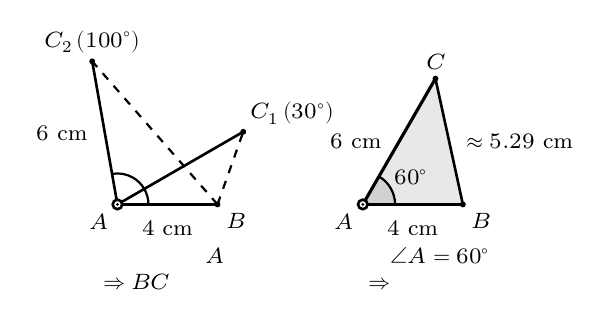
\begin{tikzpicture}[scale=0.82, every node/.style={font=\footnotesize, text=black}]
  % ផ្នែកទី១៖ ប្ដូរមុំ A (30 deg vs 100 deg)
  \begin{scope}[shift={(-2.30,0)}]
    \coordinate (A) at (0,0);
    \coordinate (B) at (1.55,0);
    \coordinate (C1) at (30:2.25);
    \coordinate (C2) at (100:2.25);
    \draw[black, line width=1.2pt] (A) -- (B) node[midway, below=2pt] {$4\text{ cm}$};
    \draw[black, line width=0.95pt] (A) -- (C1);
    \draw[black, line width=0.95pt] (A) -- (C2) node[midway, left=2.5pt] {$6\text{ cm}$};
    \draw[black, line width=0.8pt, dashed] (B) -- (C1);
    \draw[black, line width=0.8pt, dashed] (B) -- (C2);
    \draw[black, line width=0.8pt] (0.48,0) arc (0:100:0.48);
    \fill[white, draw=black, line width=0.95pt] (A) circle (2.1pt);
    \fill[black] (A) circle (0.7pt);
    \fill[black] (B) circle (1.3pt) (C1) circle (1.3pt) (C2) circle (1.3pt);
    \node[below left=2pt, inner sep=1pt] at (A) {$A$};
    \node[below right=2pt, inner sep=1pt] at (B) {$B$};
    \node[above right=1.5pt, inner sep=1pt] at (C1) {$C_1\,(30^\circ)$};
    \node[above=2pt, inner sep=1pt] at (C2) {$C_2\,(100^\circ)$};
    \node[below=12pt, align=center] at (0.78,0) {ប្តូរមុំគន្លឹះ $A$\\$\Rightarrow BC$ ប្រែប្រួល};
  \end{scope}
  % ផ្នែកទី២៖ ចាក់សោ A = 60 deg
  \begin{scope}[shift={(1.50,0)}]
    \coordinate (A) at (0,0);
    \coordinate (B) at (1.55,0);
    \coordinate (C) at (60:2.25);
    \fill[gray!18] (A) -- (B) -- (C) -- cycle;
    \fill[gray!36] (A) -- (0.50,0) arc (0:60:0.50) -- cycle;
    \draw[black, line width=0.8pt] (0.50,0) arc (0:60:0.50);
    \draw[black, line width=1.15pt] (A) -- (B) node[midway, below=2pt] {$4\text{ cm}$};
    \draw[black, line width=1.15pt] (A) -- (C) node[midway, left=2.5pt] {$6\text{ cm}$};
    \draw[black, line width=0.95pt] (B) -- (C) node[midway, right=2.5pt] {$\approx 5.29\text{ cm}$};
    \node at (29:0.86) {$60^\circ$};
    \fill[white, draw=black, line width=0.95pt] (A) circle (2.1pt);
    \fill[black] (A) circle (0.7pt);
    \fill[black] (B) circle (1.3pt) (C) circle (1.3pt);
    \node[below left=2pt, inner sep=1pt] at (A) {$A$};
    \node[below right=2pt, inner sep=1pt] at (B) {$B$};
    \node[above=2pt, inner sep=1pt] at (C) {$C$};
    \node[below=12pt, align=center] at (0.85,0) {ចាក់សោ $\angle A=60^\circ$\\$\Rightarrow$ រាងតែមួយគត់};
  \end{scope}
\end{tikzpicture}}

% ៥. E2 Explore: អន្ទាក់ ជ.ជ.ម (SSA Pendulum Arc) – ស-ខ្មៅ បន្ទាត់ច្បាស់
\newcommand{\figSSATrap}{%
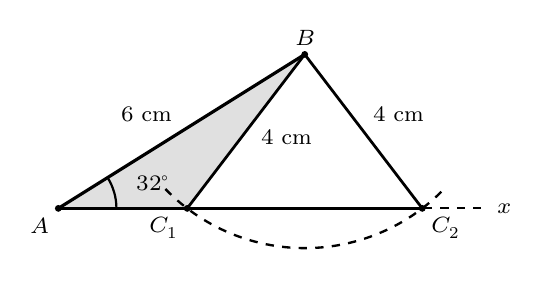
\begin{tikzpicture}[scale=0.82, every node/.style={font=\footnotesize, text=black}]
  \coordinate (A) at (0,0);
  \coordinate (B) at (3.8162, 2.3846);
  \coordinate (C1) at (1.9959, 0);
  \coordinate (C2) at (5.6365, 0);
  \coordinate (Xend) at (6.55, 0);
  \fill[gray!24] (A) -- (B) -- (C1) -- cycle;
  \fill[white] (B) -- (C1) -- (C2) -- cycle;
  \draw[black, line width=0.8pt, dashed] (A) -- (Xend) node[right=2pt] {$x$};
  \draw[black, line width=1.15pt] (A) -- (B) node[midway, above left=2pt, inner sep=1pt] {$6\text{ cm}$};
  \draw[black, line width=1.0pt] (B) -- (C1) node[midway, right=4pt, yshift=-2pt, inner sep=1pt] {$4\text{ cm}$};
  \draw[black, line width=1.0pt] (B) -- (C2) node[midway, above right=2pt, inner sep=1pt] {$4\text{ cm}$};
  \draw[black, line width=0.9pt] (A) -- (C2);
  \draw[black, line width=0.85pt, dashed] ($(B)+(-136:3.0)$) arc (-136:-44:3.0);
  \draw[black, line width=0.8pt] (0.90,0) arc (0:32:0.90);
  \node at (15:1.52) {$32^\circ$};
  \fill[black] (A) circle (1.5pt) node[below left=2pt, inner sep=1pt] {$A$};
  \fill[black] (B) circle (1.5pt) node[above=2pt, inner sep=1pt] {$B$};
  \fill[black] (C1) circle (1.5pt) node[below left=2pt, inner sep=1pt] {$C_1$};
  \fill[black] (C2) circle (1.5pt) node[below right=2pt, inner sep=1pt] {$C_2$};
\end{tikzpicture}}

% ៦. E3 Explain: ត្រីកោណប៉ុនគ្នាតាមលក្ខខណ្ឌ ជ.ម.ជ (S-A-S) – បង្វិល/ឆ្លុះ ~140° បំបែកអគតិរូបគំរូ
\newcommand{\figThmSAS}{%
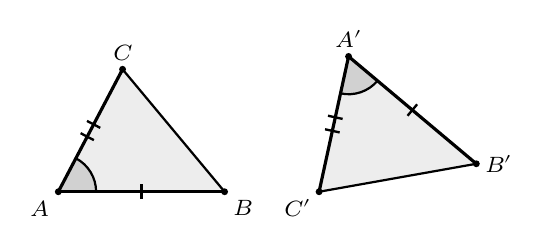
\begin{tikzpicture}[scale=0.96, every node/.style={font=\footnotesize, text=black}]
  % ត្រីកោណទី១ (ស្ដង់ដារ)
  \coordinate (A) at (0,0);
  \coordinate (B) at (2.20,0);
  \coordinate (C) at (0.85,1.62);
  \fill[gray!14] (A) -- (B) -- (C) -- cycle;
  \pic[draw=black, line width=0.8pt, fill=gray!36, angle radius=4.8mm]{angle=B--A--C};
  \draw[black, line width=0.8pt] (B) -- (C);
  \draw[black, line width=1.15pt, tk1] (A) -- (B);
  \draw[black, line width=1.15pt, tk2] (A) -- (C);
  \fill[black] (A) circle (1.3pt) (B) circle (1.3pt) (C) circle (1.3pt);
  \node[below left=2pt, inner sep=1pt] at (A) {$A$};
  \node[below right=2pt, inner sep=1pt] at (B) {$B$};
  \node[above=2pt, inner sep=1pt] at (C) {$C$};
  % ត្រីកោណទី២ (ឆ្លុះ និងបង្វិល 140 deg ដាក់បញ្ច្រាស)
  \coordinate (Ap) at (3.84,1.79);
  \coordinate (Bp) at (5.53,0.37);
  \coordinate (Cp) at (3.45,0.00);
  \fill[gray!14] (Ap) -- (Bp) -- (Cp) -- cycle;
  \pic[draw=black, line width=0.8pt, fill=gray!36, angle radius=4.8mm]{angle=Cp--Ap--Bp};
  \draw[black, line width=0.8pt] (Bp) -- (Cp);
  \draw[black, line width=1.15pt, tk1] (Ap) -- (Bp);
  \draw[black, line width=1.15pt, tk2] (Ap) -- (Cp);
  \fill[black] (Ap) circle (1.3pt) (Bp) circle (1.3pt) (Cp) circle (1.3pt);
  \node[above=2pt, inner sep=1pt] at (Ap) {$A'$};
  \node[right=2pt, inner sep=1pt] at (Bp) {$B'$};
  \node[below left=1.5pt, inner sep=1pt] at (Cp) {$C'$};
\end{tikzpicture}}

% ៧. E4 Elaborate: លំហាត់គំរូ (មុំ XOY, កន្លះបន្ទាត់ពុះ OZ, OA=OB, M in OZ) – ស-ខ្មៅ ៣ ជំហាន
\newcommand{\figModel}{%
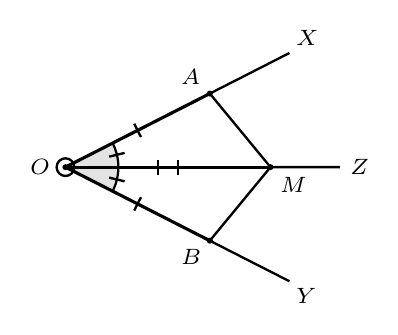
\begin{tikzpicture}[scale=0.84, every node/.style={font=\footnotesize, text=black}]
  \coordinate (O) at (0,0);
  \coordinate (X) at (27:3.80);
  \coordinate (Y) at (-27:3.80);
  \coordinate (Z) at (4.15,0);
  \coordinate (A) at (27:2.45);
  \coordinate (B) at (-27:2.45);
  \coordinate (M) at (3.10,0);
  \fill[gray!22] (O) -- (27:0.80) arc (27:-27:0.80) -- cycle;
  \draw[black, line width=0.8pt] (27:0.80) arc (27:-27:0.80);
  \draw[black, line width=0.85pt] (13.5:0.68) -- (13.5:0.92);
  \draw[black, line width=0.85pt] (-13.5:0.68) -- (-13.5:0.92);
  \draw[black, line width=0.85pt] (A) -- (X) (B) -- (Y) (M) -- (Z);
  \draw[black, line width=1.15pt, tk1] (O) -- (A);
  \draw[black, line width=1.15pt, tk1] (O) -- (B);
  \draw[black, line width=1.15pt, tk2] (O) -- (M);
  \draw[black, line width=0.85pt] (A) -- (M) -- (B);
  \draw[black, line width=0.85pt] (O) circle (3.8pt);
  \fill[black] (O) circle (1.3pt) (A) circle (1.3pt) (B) circle (1.3pt) (M) circle (1.3pt);
  \node[left=4.5pt, inner sep=1pt] at (O) {$O$};
  \node[above left=2pt, inner sep=1pt] at (A) {$A$};
  \node[below left=2pt, inner sep=1pt] at (B) {$B$};
  \node[below right=2.5pt, inner sep=1pt] at (M) {$M$};
  \node[above right=1.5pt, inner sep=1pt] at (X) {$X$};
  \node[below right=1.5pt, inner sep=1pt] at (Y) {$Y$};
  \node[right=2.5pt, inner sep=1pt] at (Z) {$Z$};
\end{tikzpicture}}

% ៨. E5 Evaluate: លំហាត់ប្រតិបត្តិ (ចំណុចឆ្លុះ A', B' ធៀបនឹង O) – ស-ខ្មៅ
\newcommand{\figPractice}{%
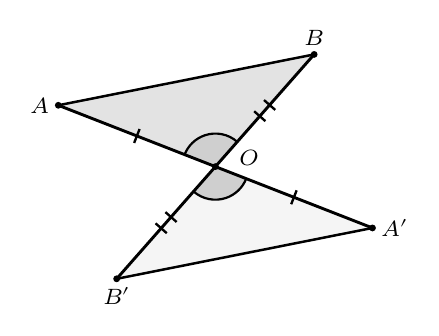
\begin{tikzpicture}[scale=0.95, every node/.style={font=\footnotesize, text=black}]
  \coordinate (O) at (0,0);
  \coordinate (A) at (-2.10, 0.82);
  \coordinate (B) at (1.32, 1.50);
  \coordinate (Ap) at (2.10, -0.82);
  \coordinate (Bp) at (-1.32, -1.50);
  \fill[gray!22] (O) -- (A) -- (B) -- cycle;
  \fill[gray!8] (O) -- (Ap) -- (Bp) -- cycle;
  \pic[draw=black, line width=0.8pt, fill=gray!38, angle radius=4.2mm]{angle=B--O--A};
  \pic[draw=black, line width=0.8pt, fill=gray!38, angle radius=4.2mm]{angle=Bp--O--Ap};
  \draw[black, line width=1.05pt, tk1] (O) -- (A);
  \draw[black, line width=1.05pt, tk1] (O) -- (Ap);
  \draw[black, line width=1.05pt, tk2] (O) -- (B);
  \draw[black, line width=1.05pt, tk2] (O) -- (Bp);
  \draw[black, line width=0.9pt] (A) -- (B) (Ap) -- (Bp);
  \fill[black] (O) circle (1.3pt) (A) circle (1.3pt) (B) circle (1.3pt) (Ap) circle (1.3pt) (Bp) circle (1.3pt);
  \node[left=2pt, inner sep=1pt] at (A) {$A$};
  \node[above=2pt, inner sep=1pt] at (B) {$B$};
  \node[right=2pt, inner sep=1pt] at (Ap) {$A'$};
  \node[below=2pt, inner sep=1pt] at (Bp) {$B'$};
  \node[inner sep=1pt] at (14:0.46) {$O$};
\end{tikzpicture}}

% ៩. ជំហានទី៥ កិច្ចការផ្ទះថ្មី៖ AB = AC, AD ពុះមុំ A, E លើ AD – ស-ខ្មៅ
\newcommand{\figHWnew}{%
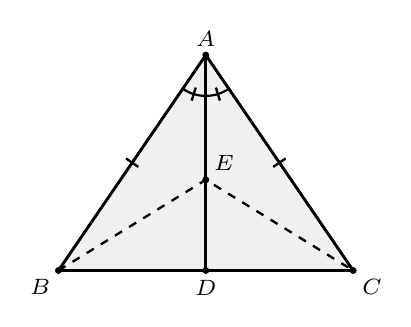
\begin{tikzpicture}[scale=0.96, every node/.style={font=\footnotesize, text=black}]
  \coordinate (A) at (0, 2.85);
  \coordinate (B) at (-1.95, 0);
  \coordinate (C) at (1.95, 0);
  \coordinate (D) at (0, 0);
  \coordinate (E) at (0, 1.20);
  \fill[gray!12] (A) -- (B) -- (C) -- cycle;
  \draw[black, line width=0.95pt] (A) -- (B) -- (C) -- cycle;
  \draw[black, line width=1.15pt] (A) -- (D);
  \draw[black, line width=0.85pt, dashed] (B) -- (E) -- (C);
  \draw[black, line width=0.95pt, tk1] (A) -- (B);
  \draw[black, line width=0.95pt, tk1] (A) -- (C);
  \draw[black, line width=0.8pt] ($(A)+(-124.38:0.54)$) arc (-124.38:-55.62:0.54);
  \draw[black, line width=0.85pt] ($(A)+(-107.19:0.45)$) -- ($(A)+(-107.19:0.63)$);
  \draw[black, line width=0.85pt] ($(A)+(-72.81:0.45)$) -- ($(A)+(-72.81:0.63)$);
  \fill[black] (A) circle (1.3pt) node[above=2pt, inner sep=1pt] {$A$};
  \fill[black] (B) circle (1.3pt) node[below left=2pt, inner sep=1pt] {$B$};
  \fill[black] (C) circle (1.3pt) node[below right=2pt, inner sep=1pt] {$C$};
  \fill[black] (E) circle (1.3pt) node[above right=2pt, inner sep=1pt] {$E$};
  \fill[black] (D) circle (1.3pt) node[below=2.5pt, inner sep=1pt] {$D$};
\end{tikzpicture}}

% ============================================================================
% ចាប់ផ្ដើមឯកសារ (Document Body)
% ============================================================================
\begin{document}
\fontsize{10pt}{15.2pt}\selectfont

% -------------------- ក្បាលកិច្ចតែងការ (Header) – តាមលំនាំ ម.ជ.ម --------------------
\begin{center}
  {\muol\fontsize{11pt}{16pt}\selectfont ព្រះរាជាណាចក្រកម្ពុជា}\\[1pt]
  {\muol\fontsize{10pt}{15pt}\selectfont ជាតិ សាសនា ព្រះមហាក្សត្រ}\\[0pt]
  \khmflourish
\end{center}

\vspace{-22pt}
{\muol\fontsize{9.5pt}{13.0pt}\selectfont
មន្ទីរអប់រំ យុវជន និងកីឡា ខេត្តកំពង់ធំ\\
ការិយាល័យអប់រំ យុវជន និងកីឡា ស្រុកកំពង់ស្វាយ\\
អនុវិទ្យាល័យព្រះក្រសាំង}

\vspace{0pt}
\begin{center}
  {\muol\fontsize{10pt}{15pt}\selectfont កិច្ចតែងការបង្រៀន}
\end{center}
\vspace{0pt}

% -------------------- ព័ត៌មានទូទៅ (Metadata) --------------------
{\renewcommand{\arraystretch}{0.92}
\hspace*{4.6cm}%
\begin{tabular}{@{}l l l@{}}
  - \hspace{0.35cm} មុខវិជ្ជា & : & គណិតវិទ្យា ថ្នាក់ទី៨ \\
  - \hspace{0.35cm} ចំណងជើងមេរៀន & : & មេរៀនទី១២ ការប្រៀបធៀបត្រីកោណ \\
  - \hspace{0.35cm} ចំណងជើងរង & : & ១.២. លក្ខខណ្ឌនៃត្រីកោណប៉ុនគ្នា \\
  & & ១.២.២ មុំមួយប៉ុនគ្នាអមដោយជ្រុងពីរប៉ុនរៀងគ្នា \\
  - \hspace{0.35cm} រយៈពេល & : & ១ ម៉ោងសិក្សា (៥០នាទី) \\
  - \hspace{0.35cm} បង្រៀនដោយ & : & ហុក ប៊ុនថែន \\
  - \hspace{0.35cm} កាលបរិច្ឆេទ & : & ថ្ងៃព្រហស្បតិ៍ ទី២៦ ខែវិច្ឆិកា ឆ្នាំ២០២៦ \\
\end{tabular}

\vspace{0pt}

% -------------------- I. វត្ថុបំណង --------------------
\textbf{I.} {\muol វត្ថុបំណង}\\[1pt]
\hspace*{0.55cm}%
\begin{tabular}{@{}l l l@{}}
  \wcirc \hspace{0.25cm} វិជ្ជាសម្បទា & : & សិស្សកំណត់បានពីលក្ខខណ្ឌនៃត្រីកោណពីរប៉ុនគ្នាក្នុងករណី មុំមួយប៉ុនគ្នាអមដោយជ្រុងពីរប៉ុនរៀងគ្នា (ជ.ម.ជ) \\
  & & និងបែងចែកភាពខុសគ្នាពីករណី ជ.ជ.ម (SSA) បានត្រឹមត្រូវ តាមពិសោធន៍ចង្កឹះគន្លឹះ ប៉ោលដៃផ្ទាល់ និង Slide ។ \\
  \wcirc \hspace{0.25cm} បំណិនសម្បទា & : & សិស្សបកស្រាយ និងប្រើប្រាស់លក្ខខណ្ឌ (ជ.ម.ជ) ដោយប្រើកាតស៊ើបអង្កេតសញ្ញាគន្លឹះ ៣ ជំហាន (ស-ខ្មៅ) \\
  & & ដើម្បីដោះស្រាយបញ្ហាជាក់ស្ដែង (វាស់ទទឹងស្រះទឹក) និងលំហាត់ប្រតិបត្តិបានច្បាស់លាស់។ \\
  \wcirc \hspace{0.25cm} ចរិយាសម្បទា & : & សិស្សមានភាពរីករាយ សហការជាក្រុម ហ៊ានទស្សន៍ទាយ សាកល្បងពិសោធន៍ និងផ្ទៀងផ្ទាត់ហេតុផល \\
  & & ដោយការទទួលខុសត្រូវជាប្រចាំ។ \\
\end{tabular}

\vspace{0pt}

% -------------------- II. សម្ភារៈឧបទេស --------------------
\textbf{II.} {\muol សម្ភារៈឧបទេស}\\[1pt]
\hspace*{0.55cm}$\bullet$ \hspace{0.35cm} សៀវភៅគោលទី៨ ចង្កឹះគន្លឹះ (4cm, 6cm) ក្រដាសស្តើង កាតស៊ើបអង្កេត ៣ ជំហាន (ស-ខ្មៅ) និង Slide Animation

\vspace{0pt}

% -------------------- III. វិធីសាស្រ្តបង្រៀន --------------------
\textbf{III.} {\muol វិធីសាស្រ្តបង្រៀន}\\[1pt]
\hspace*{0.55cm}%
\begin{tabular}{@{}l l l@{}}
  $\bullet$ \hspace{0.35cm} គោលវិធី & : \hspace{0.7cm} & សិស្សមជ្ឈមណ្ឌល \\
  $\bullet$ \hspace{0.35cm} យុទ្ធវិធីបង្រៀន & : & ស្ថាបនានិយម គម្រូ 5Es (ពិសោធន៍ផ្ទាល់ដៃ ល្បែងស៊ើបអង្កេត និងប្រកួតក្រុម) \\
\end{tabular}
}

\vspace{0pt}

% -------------------- IV. ដំណើរការបង្រៀន --------------------
\textbf{IV.} {\muol ដំណើរការបង្រៀន}

\vspace{0pt}

% ============================================================================
% តារាងដំណើរការបង្រៀន (Granular Sub-Row 3-Column Table – 50 នាទី)
% ============================================================================
\renewcommand{\arraystretch}{1.15}
\begin{longtable}{|L{5.50cm}|L{7.90cm}|L{4.80cm}|}
\hline
\rowcolor{headgray}
\multicolumn{1}{|c|}{\muol សកម្មភាពគ្រូ} &
\multicolumn{1}{c|}{\muol ខ្លឹមសារមេរៀន} &
\multicolumn{1}{c|}{\muol សកម្មភាពសិស្ស} \\
\hline
\endfirsthead

\hline
\endhead

\hline
\endfoot

\hline
\endlastfoot

% ==================== ជំហានទី១ ====================
\stepheader{ជំហានទី១ (រដ្ឋបាលថ្នាក់)}
- ពិនិត្យអវត្តមាន និងអនាម័យថ្នាក់រៀន \par
- ចាត់សិស្សជាដៃគូ ឬក្រុម ៣ នាក់ («ក្រុមវិស្វករ») និងចែកកញ្ចប់សម្ភារៈទុកលើតុ
&
\hspace*{0.3cm}- រដ្ឋបាលថ្នាក់ \par
\hspace*{0.3cm}- អនាម័យ និងសណ្ដាប់ធ្នាប់ថ្នាក់រៀន \par
\hspace*{0.3cm}- ត្រៀមក្រុមពិសោធន៍
&
- រាយការណ៍អវត្តមាន \par
- រៀបចំតុតាមដៃគូ/ក្រុម \\
\hline

% ==================== ជំហានទី២ ====================
\stepheader{ជំហានទី២ (កិច្ចការផ្ទះ + ទំនាក់ទំនងមេរៀនថ្មី)}
% --- ២.១a កំណែកិច្ចការផ្ទះ៖ ល្បែងចាប់កំហុស ---
\timenote{(កំណែកិច្ចការផ្ទះ៖ មិនឱ្យលើស 3min)} \par
- ពិនិត្យកិច្ចការផ្ទះរបស់សិស្សជាមុន \par
\ditem \textbf{ល្បែងចាប់កំហុស} ៖ បញ្ចាំងប្រធាន និងសួរបញ្ឆោតលើ Slide ៖ \par
«តើ $\ang{KBD} = \ang{ABD}$ ត្រូវឬខុស? ហេតុអ្វី?» \par
- ឱ្យដៃគូពិភាក្សា និងលើកសញ្ញាពន្យល់
&
\centerline{\redsub{កំណែកិច្ចការផ្ទះ (មេរៀនមុន ម.ជ.ម)}} \par
\hspace*{0.1cm}ត្រីកោណ $ABC$ ($AB < AC$), កន្លះបន្ទាត់ពុះ $AD$, $E \in AC$ ដែល $\ang{ADE} = \ang{ADB}$, បន្លាយ $ED$ កាត់ $AB$ ត្រង់ $K$ ។
&
- ផ្ទៀងផ្ទាត់ និងចាប់កំហុសបញ្ឆោត ($\ang{KBD} \neq \ang{ABD}$ ព្រោះជាមុំបន្ថែមគ្នា) \\[3pt]

% --- ២.១b រូបភាពកំណែកិច្ចការផ្ទះ (Isolated Row) ---
&
\cfig{\figHWold}
&
\\[3pt]

% --- ២.២a ចម្លើយកំណែកិច្ចការផ្ទះ (ក) ---
- សរសើរក្រុមដែលចាប់កំហុសបានរហ័ស និងបង្ហាញចម្លើយសង្ខេបលើ Slide
&
\centerline{\underline{ចម្លើយ}} \par
\hspace*{0.1cm}ក. ក្នុង $\tri{ABD}$ និង $\tri{AED}$ មាន \par
\hspace*{0.3cm}$\ang{BAD}=\ang{EAD}$ (ពុះមុំ) \par
\hspace*{0.3cm}$AD=AD$ (ជ្រុងរួម) \par
\hspace*{0.3cm}$\ang{ADB}=\ang{ADE}$ (សម្មតិកម្ម) \par
\hspace*{0.2cm}$\Rightarrow \tri{ABD} \cg \tri{AED}$ (ម.ជ.ម) \par
\hspace*{0.2cm}+ វិបាក ៖ $BD=ED$ និង $\ang{ABD}=\ang{AED}$ ។
&
- ផ្ទៀងផ្ទាត់ និងសរសេរហេតុផលក្រោយសមភាព \\[3pt]

% --- ២.២b ចម្លើយកំណែកិច្ចការផ្ទះ (ខ) ---
&
\hspace*{0.1cm}ខ. ក្នុង $\tri{KBD}$ និង $\tri{CED}$ មាន \par
\hspace*{0.3cm}$\ang{KBD}=180^\circ-\ang{ABD}=180^\circ-\ang{AED}=\ang{CED}$ \par
\hspace*{0.3cm}$BD=ED$ (វិបាក ក) \par
\hspace*{0.3cm}$\ang{KDB}=\ang{CDE}$ (ទល់កំពូល) \par
\hspace*{0.1cm}ដូចនេះ \graybox{$\tri{KBD} \cg \tri{CED}$ (ម.ជ.ម)} \par
\hspace*{0.2cm}$\Rightarrow KD=CD$ និង $KB=CE$ ។
&
- កត់ចំណាំដំណោះស្រាយ ក និង ខ \\[3pt]

% --- ២.៣a កាយវិការរហ័ស ១៖ មុំទល់កំពូល ---
\timenote{(រំលឹកមេរៀន៖ មិនឱ្យលើស 3min)} \par
\ditem \textbf{កាយវិការរហ័ស (ភាគ ១)} ៖ ឱ្យសិស្សធ្វើសញ្ញាខ្វែងប៊ិច ឬដៃទាំងពីរតំណាងបន្ទាត់ពីរកាត់គ្នា \par
– សំណួរ៖ តើមុំទល់កំពូលមានលក្ខណៈដូចម្ដេច?
&
\centerline{\redsub{រំលឹកមេរៀនទាក់ទងមេរៀនថ្មី}} \par
\hspace*{0.1cm}- \textbf{មុំទល់កំពូល} (\graybox{\textit{Slide Animation}})
&
- លើកដៃខ្វែងគ្នា \par
- ឆ្លើយស្រុះ៖ «មុំទល់កំពូលមានរង្វាស់ប៉ុនគ្នា!» \\[3pt]

% --- ២.៣b រូបភាពមុំទល់កំពូល (Isolated Row) ---
&
\cfig{\figVert}
\centerline{$\ang{AOB} = \ang{A'OB'}$ (មុំទល់កំពូលមានរង្វាស់ស្មើគ្នា)}
&
\\[3pt]

% --- ២.៤a កាយវិការរហ័ស ២៖ កន្លះបន្ទាត់ពុះមុំ ---
\ditem \textbf{កាយវិការរហ័ស (ភាគ ២)} ៖ ឱ្យសិស្សបត់កែងក្រដាសព្រៀងជាពីរឱ្យគែមត្រួតស៊ីគ្នា តំណាងកន្លះបន្ទាត់ពុះមុំ \par
– សំណួរ៖ តើកន្លះបន្ទាត់ពុះមុំចែកមុំយ៉ាងដូចម្ដេច?
&
\hspace*{0.1cm}- \textbf{កន្លះបន្ទាត់ពុះមុំ} (\graybox{\textit{Paper Fold}})
&
- បត់ក្រដាស \par
- ឆ្លើយ៖ «ចែកមុំជាពីរផ្នែកប៉ុនគ្នា!» \\[3pt]

% --- ២.៤b រូបភាពកន្លះបន្ទាត់ពុះមុំ (Isolated Row) ---
&
\cfig{\figBisect}
\centerline{$OZ$ ពុះ $\ang{XOY} \Rightarrow \ang{XOZ} = \ang{ZOY}$}
&
\\[3pt]

% --- ២.៥a E1 Engage: បេសកកម្មវាស់ទទឹងស្រះទឹក ---
\fiveE{E1 - Engage} \timenote{(3min)} \par
\ditem \textbf{បេសកកម្មវាស់ទទឹងស្រះ} ៖ លើករឿងពិត៖ \par
«មានបង្គោល $A$ និង $B$ នៅត្រើយម្ខាងគ្នានៃស្រះទឹក។ វិស្វករវាស់ $OA'=OA$ និង $OB'=OB$ លើដីគោក រួចវាស់បាន $A'B' = 18\text{ m}$ ហើយប្រកាសថាទទឹងស្រះ $AB = 18\text{ m}$ ដោយមិនចុះទឹក!»
&
\centerline{\redsub{ស្ថានភាពបញ្ហាពិត៖ វាស់ទទឹងស្រះដោយមិនឆ្លងទឹក}}
&
- សង្កេតរូបស្រះទឹក ភ្ញាក់ផ្អើល និងបញ្ចេញមតិទស្សន៍ទាយ \\[3pt]

% --- ២.៥b រូបភាពស្រះទឹក (Isolated Row) ---
&
\cfig{\figPondHook}
&
\\[3pt]

% --- ២.៥c E1 Engage: សំណួរចោទ និងសម្គាល់ ---
– សំណួរ៖ តើស្គាល់តែជ្រុង ២ គូ ($OA=OA', OB=OB'$) និងមុំចន្លោះ ($\ang{AOB}=\ang{A'OB'}$) គ្រប់គ្រាន់ឱ្យ $\tri{OAB}\cg\tri{OA'B'}$ ឬទេ?
&
\hspace*{0.1cm}- \textbf{សម្គាល់} ៖ ជ្រុង $OA, OB$ អមជុំវិញមុំ $\ang{AOB}$ (ទម្រង់ ជ្រុង--មុំ--ជ្រុង) ។ \par
\hspace*{0.1cm}- ទាញចំណាប់អារម្មណ៍សិស្សចូលមេរៀនថ្មី
&
- ចង់ពិសោធន៍រកការពិតដោយផ្ទាល់ដៃ \\
\hline

% ==================== ជំហានទី៣ ====================
\stepheader{ជំហានទី៣ (ខ្លឹមសារមេរៀនថ្មី)}
% --- ៣.១ ចំណងជើង និងបញ្ហាគន្លឹះ E2 ---
\fiveE{E2 - Explore} \timenote{(11min)} \par
- សរសេរចំណងជើងមេរៀនថ្មីលើក្ដារខៀន \par
\ditem បញ្ចាំងសំណួរធំលើក្ដារខៀនដើម្បីបំផុសការពិសោធន៍
&
មេរៀនទី១២ \hspace{0.15cm} {\muol ការប្រៀបធៀបត្រីកោណ (ត)} \par
១.២. លក្ខខណ្ឌនៃត្រីកោណប៉ុនគ្នា \par
១.២.២ មុំមួយប៉ុនគ្នាអមដោយជ្រុងពីរប៉ុនរៀងគ្នា (ជ.ម.ជ) \par\vspace*{2pt}
\hspace*{0.2cm}ប្រសិនបើយើងសង់ត្រីកោណពីរ ដោយស្គាល់ប្រវែងជ្រុងពីរប៉ុនរៀងគ្នា និងមុំមួយអមចន្លោះជ្រុងទាំងពីរនោះប៉ុនគ្នា តើត្រីកោណទាំងពីរនោះប៉ុនគ្នាដែរឬទេ?
&
- កត់ត្រាចំណងជើងមេរៀន \par
- ឆ្លើយតាមការយល់ឃើញ \\[3pt]

% --- ៣.២a ពិសោធន៍ទី១៖ ចង្កឹះបត់គន្លឹះ (7min) ---
\ditem \textbf{ពិសោធន៍ ១៖ ចង្កឹះបត់គន្លឹះ} \timenote{(7min)} \par
+ ចែកបន្ទះគន្លឹះ $4\text{cm}$ ($AB$) និង $6\text{cm}$ ($AC$) ភ្ជាប់ត្រង់ $A$ ។ \par
+ ឱ្យសិស្សបើក–បិទមុំ $\ang{A}$ ($30^\circ\leftrightarrow 100^\circ$) ព្រមទាំងពោល៖ \par
«ជ្រុង $BC$ ចាក់សោពេលមុំអមចន្លោះ $\ang{A}$ ចាក់សោ!»
&
\hspace*{0.1cm}- \textbf{សកម្មភាព ១} ៖ ចង្កឹះគន្លឹះ ($AB=4\text{cm}, AC=6\text{cm}$)
&
- បើក–បិទគន្លឹះ ពោលពាក្យ និងសង្កេត $BC$ ប្រែប្រួលតាមមុំ $\ang{A}$ \\[3pt]

% --- ៣.២b រូបភាពពិសោធន៍ទី១ (Isolated Row) ---
&
\cfig{\figHingeExplore}
&
\\[3pt]

% --- ៣.២c ពិសោធន៍ទី១៖ ចាក់សោមុំ & ក្រដាសស្តើងផ្ទៀងត្រួត ---
+ ចាក់សោ $\ang{A}=60^\circ$ គូស $BC$ \par
+ រួចគូរ/កាត់លើក្រដាសស្តើង \textbf{បង្វិល–ត្រឡប់ផ្ទៀងត្រួត} លើត្រីកោណក្រុមជិតខាង ។
&
+ បើ $\ang{A}$ ប្រែប្រួល $\Rightarrow BC$ ប្រែប្រួល ($3.23\text{cm} \neq 7.77\text{cm}$) \par
+ ចាក់សោ $\ang{A}=60^\circ \Rightarrow BC\approx 5.29\text{cm}$ \par
+ ក្រដាសស្តើងបង្វិល–ត្រឡប់ត្រួតស៊ីគ្នាបេះបិទ!
&
- ចាក់សោ $60^\circ$ \par
- កាត់/បង្វិលក្រដាសស្តើងផ្ទៀងត្រួតគ្នាបេះបិទ \\[3pt]

% --- ៣.៣a ពិសោធន៍ទី២៖ POE អន្ទាក់ ជ.ជ.ម (4min) ---
\ditem \textbf{ពិសោធន៍ ២៖ POE អន្ទាក់ ជ.ជ.ម} \timenote{(4min)} \par
+ \textbf{ទស្សន៍ទាយ (P)}៖ ដឹង $AB=6\text{cm}, BC=4\text{cm}, \ang{A}=32^\circ$ (មុំមិននៅចន្លោះ) \par
– សំណួរ៖ តើបង្កើតបានប៉ុន្មានត្រីកោណ?
&
\hspace*{0.1cm}- \textbf{សកម្មភាព ២} ៖ ហេតុអ្វីមុំត្រូវតែ«អមចន្លោះជ្រុង»?
&
- ទស្សន៍ទាយចំនួនត្រីកោណមុនពេលសាកល្បង \\[3pt]

% --- ៣.៣b រូបភាពអន្ទាក់ ជ.ជ.ម (Isolated Row) ---
&
\cfig{\figSSATrap}
&
\\[3pt]

% --- ៣.៣c ពិសោធន៍ទី២៖ យោលប៉ោលដៃផ្ទាល់ (Observe-Explain) ---
+ \textbf{សង្កេត–ពន្យល់ (O–E)}៖ ដៃផ្ទាល់យោលបន្ទះ $BC=4\text{cm}$ ជុំវិញ $B$ កាត់ $Ax$ (២ ចំណុច) \textit{មុន} បញ្ចាំង Slide សំយោគ។
&
យោលប៉ោល $BC=4\text{cm}$ កាត់ $Ax$ ត្រង់ $C_1, C_2$ ៖ \par
\graybox{$\tri{ABC_1} \not\cg \tri{ABC_2}$ (ជ.ជ.ម មិនអាចប្រើបាន!)}
&
- យោលផ្ទាល់ដៃ ឃើញ $C_1, C_2$ រួចពន្យល់មូលហេតុខុស \\[3pt]

% --- ៣.៤a E3 Explain: ទ្រឹស្ដីបទ S-A-S & គោលការណ៍កំពូលរួម ---
\fiveE{E3 - Explain} \timenote{(6min)} \par
\ditem បញ្ជាកាយវិការបើក–ចាក់សោ S--A--S ជួយសិស្សបង្គុំទ្រឹស្ដីបទ និងបង្ហាញ \textbf{ធនាគារហេតុផល} \par
– សំណួរ \cnum{1}៖ តើយើងទាញជាទ្រឹស្ដីបទរួមដូចម្ដេច?
&
\textbf{ទ្រឹស្ដីបទ (ជ.ម.ជ) ៖} \par
ត្រីកោណពីរប៉ុនគ្នា កាលណាវាមានមុំមួយប៉ុនគ្នា អមដោយជ្រុងពីរប៉ុនរៀងគ្នា ។ \par
\redsub{\textbf{គោលការណ៍កំពូលរួម} ៖} កំពូលមុំត្រូវជាប់ចន្លោះជ្រុងទាំងពីរ (S--A--S) ទោះរូបបង្វិល–ឆ្លុះ $140^\circ$ ក៏ផ្ទៀងតាមលំដាប់កំពូល ។
&
- បង្គុំទ្រឹស្ដីបទ ជ.ម.ជ និងចំណាំកំពូលរួមលើរូបបង្វិល \\[3pt]

% --- ៣.៤b រូបភាពទ្រឹស្ដីបទ ជ.ម.ជ (Isolated Row) ---
&
\cfig{\figThmSAS}
&
\\[3pt]

% --- ៣.៥a E3 Explain: តារាងសម្មតិកម្ម-សន្និដ្ឋាន-វិបាក (Isolated Row) ---
– សំណួរ \cnum{2}៖ ពេល $\tri{ABC} \cg \tri{A'B'C'}$ តើធាតុ ៣ នៅសល់យ៉ាងណា? តើ $=$ និង $\cg$ ខុសគ្នាដូចម្ដេច?
&
\cfig{%
\setlength{\tabcolsep}{2.2pt}%
\renewcommand{\arraystretch}{1.12}%
\begin{tabular}{|c|c|c|}
  \hline
  \cellcolor{headgray} សម្មតិកម្ម (ជ.ម.ជ) & \cellcolor{headgray} សន្និដ្ឋាន & \cellcolor{headgray} វិបាក \\
  \hline
  $AB = A'B'$ & & $\ang{B} = \ang{B'}$ \\
  $\ang{A} = \ang{A'}$ & $\tri{ABC} \cg \tri{A'B'C'}$ & $BC = B'C'$ \\
  $AC = A'C'$ & {\footnotesize (តាមលក្ខខណ្ឌ ជ.ម.ជ)} & $\ang{C} = \ang{C'}$ \\[2pt]
  \hline
\end{tabular}%
}
&
- សង្កេតតារាងសម្មតិកម្ម សន្និដ្ឋាន និងវិបាក \\[3pt]

% --- ៣.៥b ធនាគារហេតុផល & សម្គាល់ = vs \cong ---
- សង្ខេបធនាគារហេតុផល \cnum{1}--\cnum{5} និងបញ្ជាក់ភាពខុសគ្នារវាង $=$ និង $\cg$
&
\textbf{ធនាគារហេតុផល៖} \par
\cnum{1} បម្រាប់ \quad \cnum{2} មុំទល់កំពូល/ពុះមុំ \quad \cnum{3} ជ្រុងរួម \par
\cnum{4} ជ.ម.ជ $\rightarrow$ \cnum{5} ធាតុត្រូវគ្នា ។ \par
\textbf{សម្គាល់}៖ $=$ ប្រើសម្រាប់ប្រវែង/រង្វាស់ស្មើគ្នា និង $\cg$ សម្រាប់ត្រីកោណប៉ុនគ្នា ។
&
- កត់ចំណាំវិបាក ធនាគារ \cnum{1}--\cnum{5} និងភាពខុសគ្នា $=$ vs $\cg$ \\
\hline

% ==================== ជំហានទី៤ ====================
\stepheader{ជំហានទី៤ (ពង្រីកចំណេះដឹង)}
% --- ៤.១a E4 Elaborate: កាតស៊ើបអង្កេតសញ្ញាគន្លឹះ ៣ ជំហាន ---
\fiveE{E4 - Elaborate} \timenote{(10min)} \par
\ditem \textbf{កាតស៊ើបអង្កេតសញ្ញាគន្លឹះ ៣ ជំហាន} (ស-ខ្មៅ)៖ ចង្អុលម្រាមដៃមុនសរសេរ៖
&
{\muol លំហាត់គំរូ} \textbf{:} គេឱ្យ $\ang{XOY}$ និងកន្លះបន្ទាត់ពុះ $OZ$ ។ លើ $OX, OY$ ដៅ $A, B$ ដែល $OA = OB$ និងដៅចំណុច $M \in OZ$ ។
&
- អានប្រធានលើកាត ស-ខ្មៅ \\[3pt]

% --- ៤.១b គូសសញ្ញា ៣ ជំហាន & សំណួរ ក ខ ---
\cnum{1} ចង្អុលអូស + គូស $|$ លើ $OA=OB$ \par
\cnum{2} ចង្អុលបត់ + ព័ទ្ធ $O$ និងធ្នូ $\ang{AOM}=\ang{BOM}$ \par
\cnum{3} ចង្អុលអូស + គូស $\parallel$ លើជ្រុងរួម $OM=OM$
&
\hspace*{0.2cm}ក. ប្រៀបធៀបត្រីកោណ $OMA$ និង $OMB$ ។ \par
\hspace*{0.2cm}ខ. ទាញបញ្ជាក់ថា $MA = MB$ និង $\ang{OAM} = \ang{OBM}$ ។
&
- ចង្អុលអូស–បត់ និងគូសសញ្ញា ៣ ជំហានលើកាត \\[3pt]

% --- ៤.១b រូបភាពលំហាត់គំរូ (Isolated Row) ---
&
\cfig{\figModel}
&
\\[3pt]

% --- ៤.១c ផែនការ P2 ---
- \textbf{ផែនការ (P2)}៖ រកត្រីកោណផ្ទុក $MA, MB$ រួចតភ្ជាប់តាម \cnum{1}--\cnum{4} ឆ្លងត្រីកោណ
&
\textbf{វិភាគផែនការ៖} រក $\tri{OMA}$ និង $\tri{OMB}$ ដែលផ្ទុក $MA, MB$ ។
&
- ផ្គូផ្គងឆ្លងត្រីកោណ៖ $OA$ ទល់ $OB$, $OM$ រួម និង $\ang{AOM}=\ang{BOM}$ \\[3pt]

% --- ៤.២ ចម្លើយលំហាត់គំរូ (ក) ---
\ditem ពន្យល់ផែនទី «កាតតុលាការ ជ.ម.ជ»៖ \par
\cnum{1} ចង្អុល/គូស $|$ និង $\parallel$ លើជ្រុងស្មើ ២ គូ \par
\cnum{2} ចង្អុល/ព័ទ្ធកំពូលរួម $O$ និងធ្នូមុំចន្លោះ \par
\cnum{3} ផ្ទៀងលេខ \cnum{1}--\cnum{3} ឆ្លងត្រីកោណ \par
\cnum{4} សន្និដ្ឋាន \cnum{4} ជ.ម.ជ $\rightarrow$ \cnum{5} ទាញវិបាក
&
\centerline{\underline{\redsub{ចម្លើយ (កាតភស្តុតាង)}}} \par
ក. ក្នុង $\tri{OMA}$ និង $\tri{OMB}$ មាន \par
\hspace*{0.30cm}$OA = OB$ (\cnum{1} បម្រាប់/សម្មតិកម្ម) \par
\hspace*{0.30cm}$\ang{AOM} = \ang{BOM}$ (\cnum{2} $OM$ ពុះ $\ang{XOY}$) \par
\hspace*{0.30cm}$OM = OM$ (\cnum{3} ជ្រុងរួម / Reflexive) \par
\hspace*{0.20cm}ដូចនេះ \graybox{$\tri{OMA} \cg \tri{OMB}$ (\cnum{4} ជ.ម.ជ)}
&
- ផ្ទៀងផ្ទាត់ ៣ បន្ទាត់ដាក់លេខ \cnum{1}--\cnum{4} ជាមួយដៃគូ និងសួរដេញដោល \\[3pt]

% --- ៤.៣ ចម្លើយលំហាត់គំរូ (ខ) & POE Looking-Back ៣០ វិនាទី ---
\ditem នាំទាញវិបាក (ខ) រួចដាក់ \textbf{POE ពិនិត្យក្រោយ (30s)}៖ \par
«បើ $M$ រំកិលលើ $OZ$ តើអ្វីប្រែ ($OM, MA$) និងអ្វីថេរ ($OA=OB, \ang{AOM}=\ang{BOM}, OM=OM$)? តើ \cnum{1}--\cnum{5} នៅដដែលឬ?»
&
ខ. ដោយ $\tri{OMA} \cg \tri{OMB}$ គេទាញបាន \cnum{5} ធាតុត្រូវគ្នា៖ \par
\hspace*{0.20cm}\graybox{$MA = MB$ និង $\ang{OAM} = \ang{OBM}$ ពិត} \par
\timenote{POE ៣០វិ.៖ ទោះ $M$ រំកិលលើ $OZ$ ក៏លក្ខខណ្ឌថេរ \cnum{1}--\cnum{5} នៅពិតជានិច្ច!}
&
- ញែកអ្វីប្រែ vs អ្វីថេរ និងបញ្ជាក់គ្រប់ចំណុចលើបន្ទាត់ពុះមុំ $MA=MB$ \\[3pt]

% --- ៤.៤a E5 Evaluate: Relay Proof Race ៣ តួនាទី ---
\fiveE{E5 - Evaluate} \timenote{(10min)} \par
\ditem {\muol លំហាត់ប្រតិបត្តិ} (\textbf{Relay Proof Race ៣ តួនាទី}) \par
គេមាន $\tri{AOB}$ ។ $A', B'$ ជាចំណុចឆ្លុះនៃ $A, B$ ធៀប $O$ ។ បង្ហាញ $\tri{OAB}\cg\tri{OA'B'}$ រួចទាញ $AB=A'B'$ \textbf{ដោះស្រាយទទឹងស្រះ E1} ។ \par
\redsub{(ក្រុម ៣ នាក់ បន្តដៃគ្នា ៣០វិនាទី/ម្នាក់)}
&
{\muol ចម្លើយលំហាត់ប្រតិបត្តិ} \par
បង្ហាញថា $\tri{OAB} \cg \tri{OA'B'}$ និងទាញ $AB = A'B'$
&
- អានប្រធាន និងបែងចែកតួនាទី ១--៣ ក្នុងក្រុម \\[3pt]

% --- ៤.៤b រូបភាពលំហាត់ប្រតិបត្តិ (Isolated Row) ---
&
\cfig{\figPractice}
&
\\[3pt]

% --- ៤.៥a ដំណោះស្រាយលម្អិត៖ វេន ១--២ (Pause-Ask) ---
- ចាត់វេន Relay (\textbf{Pause-Ask} មុនគូស/ផ្ទេរវេន)៖ \par
\cnum{1} អ្នកទី១ (\textbf{Pause-Ask})៖ ពន្យល់មាត់ផ្ទាល់មុនគូស (ចាប់ \cnum{2} $\ang{AOB}=\ang{A'OB'}$, \textbf{ហាមគូស $AB=A'B'$}) ព័ទ្ធ $O$ \par
\cnum{2} អ្នកទី២៖ ផ្ទៀង $O$ ចន្លោះជ្រុង សរសេរ \cnum{1}--\cnum{4}
&
ក្នុង $\tri{OAB}$ និង $\tri{OA'B'}$ មាន \par
\hspace*{0.25cm}$OA = OA'$ (\cnum{1} $A'$ ឆ្លុះ $A$ ធៀប $O$) \par
\hspace*{0.25cm}$\ang{AOB} = \ang{A'OB'}$ (\cnum{2} មុំទល់កំពូល) \par
\hspace*{0.25cm}$OB = OB'$ (\cnum{1} $B'$ ឆ្លុះ $B$ ធៀប $O$)
&
{\muol ចម្លើយរំពឹងទុកទី១} \par
ក្នុង $\tri{OAB}, \tri{OA'B'}$៖ \par
$OA = OA'$ (\cnum{1} ឆ្លុះធៀប $O$) \par
$\ang{AOB} = \ang{A'OB'}$ (\cnum{2} ទល់កំពូល) \par
$OB = OB'$ (\cnum{1} ឆ្លុះធៀប $O$) \\[3pt]

% --- ៤.៥b ដំណោះស្រាយលម្អិត៖ វេន ៣ (Pause-Review) ---
\cnum{3} អ្នកទី៣ (\textbf{Pause-Review})៖ ផ្ទៀងលំដាប់ $O\to A\to B$ ទល់ $O\to A'\to B'$ ទាញ $AB=A'B'$
&
សន្និដ្ឋាន $\tri{OAB} \cg \tri{OA'B'}$ (\cnum{4} ជ.ម.ជ)
&
$\Rightarrow \tri{OAB} \cg \tri{OA'B'}$ (\cnum{4} ជ.ម.ជ) \par
វិបាក \cnum{5}៖ $AB = A'B'$ \\[3pt]

% --- ៤.៥c ចម្លើយរំពឹងទុកទី២ ---
- សង្កេតក្រុមដែលសរសេរតាមលំដាប់ត្រីកោណឆ្លុះចាប់ផ្ដើមមុន
&
បញ្ជាក់លំដាប់កំពូល $O \leftrightarrow O$, $A \leftrightarrow A'$, $B \leftrightarrow B'$ ។
&
{\muol ចម្លើយរំពឹងទុកទី២} \par
ពិនិត្យ $\tri{OA'B'}$ និង $\tri{OAB}$៖ \par
$OA' = OA$ (\cnum{1} បម្រាប់ឆ្លុះ), $OB' = OB$ (\cnum{1}) \par
$\ang{A'OB'} = \ang{AOB}$ (\cnum{2} ទល់កំពូល) \par
$\Rightarrow \tri{OA'B'} \cg \tri{OAB}$ (\cnum{4} ជ.ម.ជ) \\[3pt]

% --- ៤.៦a បិទបញ្ចប់ស្រះទឹក E1 ---
- បិទបញ្ចប់បេសកកម្ម E1 ទទឹងស្រះទឹកប្រយោល
&
វិបាក \cnum{5}៖ $AB = A'B'$, $\ang{OAB}=\ang{OA'B'}$, $\ang{OBA}=\ang{OB'A'}$ \par
ដូចនេះ \graybox{ទទឹងស្រះ $AB=A'B'=18\text{ m}$ ពិត!}
&
- ផ្ទៀងលំដាប់កំពូល ប្រកាស $18\text{ m}$ \\[3pt]

% --- ៤.៦b មេដៃបញ្ឆោត ៦០–៩០ វិនាទី (៤ កាត ស-ខ្មៅ) ---
- លេង \textbf{មេដៃបញ្ឆោត (60--90s)}៖ ចង្អុលខ្យល់ S--A--S មុនលើកមេដៃ/ខ្វែងដៃលើ \textbf{៤ កាត ស-ខ្មៅ}៖ \par
(១) ជ.ម.ជ $140^\circ$, (២) ជ.ជ.ម មុំក្រៅ, \par
(៣) គ្មានសញ្ញាស្មានភ្នែក, (៤) ម.ម.ម/លំដាប់ខុស $\tri{ABC}\cg\tri{FED}$ + ម្រាម ១--៣
&
\textbf{សង្ខេបតេស្ត ៤ កាត៖} (១) \ding{51} ជ.ម.ជ; (២) \ding{55} មុំក្រៅ; (៣) \ding{55} គ្មានសញ្ញា; (៤) \ding{55} កំពូលខុស ។
&
- ចង្អុលខ្យល់ លើកមេដៃ/ខ្វែងដៃ ៤ កាត និងម្រាម ១--៣ \\
\hline

% ==================== ជំហានទី៥ ====================
\stepheader{ជំហានទី៥ (កិច្ចការផ្ទះ + បណ្ដាំផ្ញើ)}
% --- ៥.១ កិច្ចការផ្ទះ (ប្រធាន) ---
\timenote{(មិនឱ្យលើស 2min)} \par
\ditem បញ្ចាំងកិច្ចការផ្ទះលើ Slide (ប្រើធនាគារ \cnum{1}--\cnum{5}) ផ្ញើចូល Telegram និង Google Classroom
&
\centerline{\muol កិច្ចការផ្ទះ} \par
គេមាន $\tri{ABC}$ ($AB = AC$), កន្លះបន្ទាត់ពុះ $AD$ នៃ $\ang{BAC}$ ($D \in BC$), និង $E \in AD$ ($E \neq A, D$) ។
&
- កត់ត្រា \\[3pt]

% --- ៥.២ សំណួរ ក និង ខ ---
- ដាស់តឿនសិស្សឱ្យគូសសញ្ញា $|, \parallel$ និងផ្ទៀងលំដាប់កំពូល
&
ក. បង្ហាញថា $\tri{ABD} \cg \tri{ACD}$ រួចទាញថា $DB = DC$ និង $\ang{ADB} = \ang{ADC}$ ។ \par
ខ. ស្រាយបញ្ជាក់ថា $\tri{BDE} \cg \tri{CDE}$ រួចទាញថា $EB = EC$ និង $\ang{DBE} = \ang{DCE}$ ។
&
- ស្ដាប់ណែនាំ និងកត់សំណួរ ក--ខ \\[3pt]

% --- ៥.៣a រូបភាពកិច្ចការផ្ទះ (Isolated Row) ---
&
\cfig{\figHWnew}
&
\\[3pt]

% --- ៥.៣b បណ្ដាំផ្ញើ ---
\ditem ចេញលេង និងត្រឡប់ផ្ទះ គោរពច្បាប់ចរាចរណ៍ ជួយការងារឪពុកម្ដាយ និងកុំភ្លេចធ្វើកិច្ចការផ្ទះ
&
- ផ្ដាំផ្ញើការងារផ្ទះ និងវិន័យសុវត្ថិភាពតាមផ្លូវ
&
- បាទ/ចាស៎លោកគ្រូ \\
\end{longtable}

% -------------------- កាលបរិច្ឆេទ និងហត្ថលេខា (Date & Signature) --------------------
\vspace{2pt}
\hfill
\begin{minipage}{9.8cm}
  {\centering
    ថ្ងៃព្រហស្បតិ៍ ២រោច ខែកត្តិក ឆ្នាំមមី អដ្ឋស័ក ពុទ្ធសករាជ ២៥៧០\\[2pt]
    ត្រូវនឹងថ្ងៃទី២៦ ខែវិច្ឆិកា ឆ្នាំ២០២៦\\[3pt]
    {\muol គ្រូបង្រៀន}\par}
  \vspace{32pt}
  \hfill{\muol ហុក ប៊ុនថែន}\hspace*{1.4cm}
\end{minipage}

\end{document}
